The data for this study includes post-vaccination HI titres of subjects who were followed for up to one year for flu infection. The infection status was determined by PCR which was done for everyone who experienced symptoms. This data is shown in Figure \ref{fig:kiddyvax-main-titre}.

\begin{figure}[htp]
	\centering
	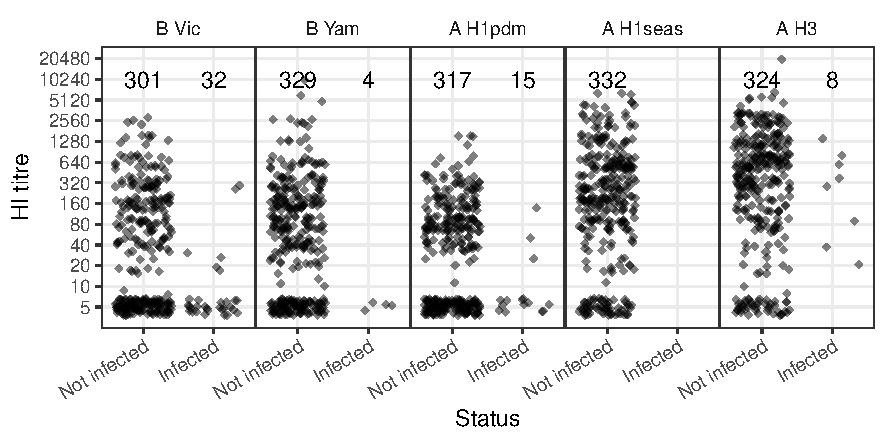
\includegraphics[width=1\textwidth]{../data-plot/kiddyvax-main-titre.pdf}
	\caption{
	Kiddyvax study data. Post-vaccination titres are shown for those who got infected (PCR-confirmed symptomatic infection) over the course of the study and those who did not. Panels correspond to the five tested viruses: B Victoria, B Yamagata, A H1pdm, A H1 seasonal, A H3.
	}
	\label{fig:kiddyvax-main-titre}
\end{figure}

Analyses were done on the data for B Vic and A(H1pdm) viruses in the same way as for the Ha Nam data with the addition of the Cox proportional hazards model.
